\documentclass[8pt]{beamer}

\usepackage{amsfonts}
\usepackage{subfiles}
\usepackage[T2A]{fontenc}
\usepackage[utf8]{inputenc}
\usepackage[russian]{babel}

\usepackage{amsmath, amsfonts, amssymb, amsthm, mathtools, mathrsfs}
\usepackage{wasysym, dsfont}
\usepackage{graphicx}
\usepackage{float}
\usepackage{wrapfig}

\usepackage{caption}
\usepackage{subcaption}
\usepackage{longtable}
% \usepackage{subfigure}

\usepackage{multicol}
\DeclareMathOperator*{\argmax}{\arg\!\max}
\DeclareMathOperator*{\argmin}{\arg\!\min}

\mode<presentation>
{
	\usetheme{boxes}
	\beamertemplatenavigationsymbolsempty
	
	\setbeamertemplate{footline}[page number]
	\setbeamersize{text margin left=1.5em, text margin right=2.0em}
}
\newcommand\blfootnote[1]{%
	\begingroup
	\renewcommand\thefootnote{}\footnote{#1}%
	\addtocounter{footnote}{-1}%
	\endgroup
}
\newcommand\FontUP{\fontsize{10}{12}\selectfont}


\title[]{Ускорение семплирования из диффузионных моделей с использованием состязательных сетей}
\author{Охотников Никита Владимирович}
\institute{МФТИ}
\date{2023}


\begin{document}

{
\begin{frame}
  \titlepage
\end{frame}
}

\begin{frame}
	\frametitle{Цели исследования}
	
	\begin{columns}
		\begin{column}{0.9\textwidth}
	
			\begin{block}{Цель}
				\smallskip
			Исследовать способы моделирования мультимодального распределения при генеративном моделировании с помощью диффузионного процесса
			\end{block}	
			\vfill
			\begin{block}{Проблема}
					\smallskip
				Стандартный диффузионный процесс моделирует унимодальное распределение при обратном проходе. Процесс семплирования из стандартной модели требует длительного времени
			\end{block}	
			\vfill
			\begin{block}{Предлагается}
				\smallskip
				Модифицировать классическую диффузионную модель для существенного ускорения процесса семплирования
			\end{block}	
			\vfill
			\begin{block}{Решение}
				\smallskip
				Использовать неявную генеративную модель -- состязательную сеть -- на каждом шаге диффузионного процесса Необходимо
				рассмотреть различные постановки минимизационной задачи для используемой модели
			\end{block}	
	     \end{column}
	\end{columns}


\end{frame}

\begin{frame}
	\frametitle{Литература}
	\FontUP
	\begin{itemize}
		\item Jonathan Ho, Ajay Jain, and Pieter Abbeel. Denoising diffusion probabilistic models, 2020
		\medskip
		\item Zhisheng Xiao, Karsten Kreis, and Arash Vahdat. Tackling the generative learning trilemma with denoising diffusion gans, 2021.
		\medskip
		\item Alex Nichol and Prafulla Dhariwal. Improved denoising diffusion probabilistic models, 2021.
		\medskip
		\item Sebastian Nowozin, Botond Cseke, and Ryota Tomioka. f-gan: Training generative neural samplers using
		variational divergence minimization, 2016.
		\medskip
		\item Martin Arjovsky, Soumith Chintala, and L?on Bottou. Wasserstein gan, 2017.
	\end{itemize}
	
\end{frame}


	%\setlength{\footskip}{1.8cm}
\begin{frame}
	\frametitle{Неявное моделирование обратного диффузионного процесса}


	\begin{columns}
		\begin{column}{0.5\textwidth}
			\begin{block}{Диффузионный процесс}
				\begin{itemize}
				
					\item Прямой: 
					\begin{equation*}
					q(\textbf{x}_t|\textbf{x}_{t-1}) = \mathcal{N}(\textbf{x}_t; \textbf{x}_{t-1}\sqrt{1-\beta_t}, \beta_t 	\textbf{I})
					\end{equation*}
					где $t = \overline{0,T}$, $\textbf{x}_0$ -- семпл из исходного распределения, $\textbf{x}_t$ -- семпл на шаге $t$, $\beta_t\in (0,1)$\\
					
					\item Обратный: 
					\begin{equation*}
						p_{\boldsymbol{\theta}}(\textbf{x}_{t-1}|\textbf{x}_t)\!\! \underset{\text{T} \gg 1}{ \approx}\!\!\! \mathcal{N}(\textbf{x}_{t-1};\mu_{\boldsymbol{\theta}}(\textbf{x}_t, t), \Sigma_{\boldsymbol{\theta}}(\textbf{x}_t, t))
					\end{equation*}
			
				\end{itemize}
			\end{block}		
		\end{column}
		
		\begin{column}{0.55\textwidth} 
				\begin{figure}[h!]
						\begin{flushright}
							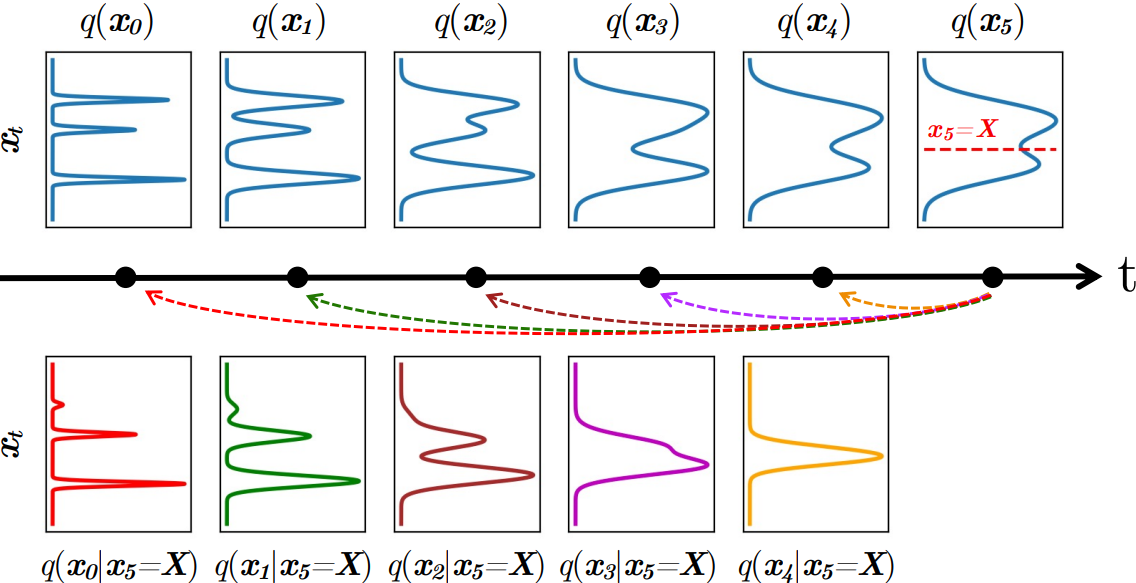
\includegraphics[width=0.97\textwidth]{figures/distributions.png}
						\end{flushright}	
				\end{figure}
	
		\end{column}
	\end{columns}


\begin{columns}
	\begin{column}{0.4\textwidth}
		
		\begin{block}{Основные предположения}
			
			\begin{itemize}	
				\item Марковость обратного процесса
				\item Нормальность и следовательно унимодальность $p_{\boldsymbol{\theta}}(\textbf{x}_{t-1}|\textbf{x}_t)$
			\end{itemize}
		
		\end{block}
	
	\end{column}
	
	\begin{column}{0.57\textwidth}  
			\begin{block}{Предложение}
				\begin{itemize}
					\item Использовать неявную модель для восстановления распределения
				\end{itemize}
			\end{block}	
		\begin{block}{Мотивация}
			\begin{itemize}
				\item Моделирование мультимодального распределения для существенного уменьшения T
			\end{itemize}
		\end{block}	
	\end{column}
\end{columns}
			\blfootnote{\url{https://doi.org/10.48550/arxiv.2112.07804}}
\end{frame}


\begin{frame}
		\frametitle{Диффузионная модель}
		\begin{block}{Описание}
		В основе модели лежит постепенное добавление случайного нормального шума с коэффициентом $\beta_t\in (0,1)$ в семпл $\textbf{x}_0$ из исходного распределения в прямом процессе и постепенное восстановление распределения в обратном. 
		\end{block}
	\begin{columns}
		
		\begin{column}{0.5\textwidth}
			\begin{block}{Прямой процесс}
				\begin{equation*}
					q(\textbf{x}_t|\textbf{x}_{t-1}) = \mathcal{N}(\textbf{x}_t; \textbf{x}_{t-1}\sqrt{1-\beta_t}, \beta_t 	\textbf{I})
				\end{equation*}
					где $t = \overline{0,T}$, $\textbf{x}_t$ -- семпл на шаге $t$.
				В таком случае, принимая $\alpha_t  = 1 - \beta_t,~\overline{\alpha_t} = \prod_{i=1}^t \alpha_i$ можно записать:
				\begin{equation*}
					q(\textbf {x}_t | \textbf{x}_0 ) = \mathcal{N} (\textbf{x}_t; \sqrt{\overline{\alpha_t}} \textbf{x}_0, (1-\overline{\alpha_t}) \textbf{I})
				\end{equation*}
				Таким образом, при достаточно больших $T$ со сколь угодно большой точностью $\textbf{x}_T\sim \mathcal{N}(0, \textbf{I})$, а значит обратный процесс начинается с нормального шума.				
			\end{block}  	 
	\end{column}

		\begin{column}{0.52\textwidth}
			\begin{block}{Обратный процесс}
				В приближении $T\gg 1$ распределение каждого следующего семпла в обратном процессе обусловлено только на предыдущий, а также нормально.
				\begin{equation*}
					p_{\boldsymbol{\theta}}(\textbf{x}_{t-1}|\textbf{x}_t)\!\! \underset{\text{T} \gg 1}{ \approx}\!\!\! \mathcal{N}(\textbf{x}_{t-1};\mu_{\boldsymbol{\theta}}(\textbf{x}_t,t), \Sigma_{\boldsymbol{\theta}}(\textbf{x}_t, t))
				\end{equation*}
			Если $\textbf{X}  = (\textbf{x}_0^1\dots\textbf{x}_0^n)\sim p_0(\textbf{x})$, то из метода максимального правдоподобия:
			\begin{equation*}
				{\boldsymbol{\theta}}^* =\argmax\limits_{{\boldsymbol{\theta}}} p(\textbf{X}|{\boldsymbol{\theta}}) = \argmax\limits_{{\boldsymbol{\theta}}} \sum\limits_{i=1}^n \log{p(\textbf{x}_0^i|{\boldsymbol{\theta}})}
			\end{equation*}			
			\end{block}
		\end{column}
	\end{columns}
\medskip
После некоторых математических преобразований получаем минимизационную задачу:
 \begin{equation*}
	\sum\limits_{t=1}^n \mathbb{E}_{\textbf{x}_1\dots \textbf{x}_T} KL\left(q(\textbf{x}_{t-1}|\textbf{x}_t, \textbf{x}_0)~||~p_{\boldsymbol{\theta}}(\textbf{x}_{t-1}|\textbf{x}_t)  \right) \xrightarrow[{\boldsymbol{\theta}}]{}\min
\end{equation*}
\blfootnote{\url{https://doi.org/10.48550/arxiv.2006.11239}}

\end{frame}

\begin{frame}
	\frametitle{Постановка задачи}
		\begin{block}{Проблема}
			При существенном уменьшении числа шагов обратного диффузионного процесса ($T\gtrsim 1$) предположения марковости и тем более нормальности $p_{\boldsymbol{\theta}}(\textbf{x}_{t-1}|\textbf{x}_t)$ очевидно не верны. Кроме того, $p_{\boldsymbol{\theta}}(\textbf{x}_{t-1}|\textbf{x}_t)$ мультимодальное.
		\end{block}
	
		\begin{block}{Задача}
			Предложить неявную модель для аппроксимации мультимодального распределения в обратном процессе. 
		\end{block}
	
	\begin{block}{Метод}
			По аналогии с классической диффузионной моделью будем минимизировать некоторую меру близости между распределениями $\textbf{D}_{adv}$, но при помощи неявной модели
			 \begin{equation*}
			\sum\limits_{t=1}^n \mathbb{E}_{\textbf{x}_1\dots \textbf{x}_T} \textbf{D}_{adv}\left(q(\textbf{x}_{t-1}|\textbf{x}_t, \textbf{x}_0)~||~p_{\boldsymbol{\theta}}(\textbf{x}_{t-1}|\textbf{x}_t)  \right) \xrightarrow[{\boldsymbol{\theta}}]{}\min
		\end{equation*}
			где $\textbf{D}_{adv}$, в случае состязательных сетей, есть некоторая f-дивергенция или метрика Вассерштайна.
		\end{block}

\end{frame}


\begin{frame}
	\frametitle{Введение GAN моделей}
	\begin{block}{Дискриминатор}
		Зададим дискриминатор как $\textbf{D}_{\boldsymbol{\varphi}}(\textbf{x}_{t-1}, \textbf{x}_t, t)$, где ${\boldsymbol{\varphi}}$ -- обучаемые параметры.\\
		Для начала используем схему тренировки стандартного GAN\footnote{\url{https://doi.org/10.48550/arxiv.1406.2661}}, как ранее было предложено\footnote{\url{https://doi.org/10.48550/arxiv.2112.07804}}, тогда задача минимизации для дискриминатора:
		$$  \min\limits_{\boldsymbol{\varphi}}\sum\limits_{t\geqslant 1}^n \mathbb{E}_{q(\textbf{x}_t)}[\mathbb{E}_{q(\textbf{x}_{t-1}|\textbf{x}_t)}[-\log{ (\textbf{D}_{\boldsymbol{\varphi}}(\textbf{x}_{t-1}, \textbf{x}_t, t) ) }] + \mathbb{E}_{p_{\boldsymbol{\theta}}(\textbf{x}_{t-1}|\textbf{x}_t)}[-\log{  (1 - \textbf{D}_{\boldsymbol{\varphi}}(\textbf{x}_{t-1}, \textbf{x}_t, t))  }]]$$
		\end{block}
		
	\begin{block}{Генератор}
		Введем генератор $\textbf{G}_{\boldsymbol{\theta}}(\textbf{x}_{t-1}^{fake}, \textbf{z}, t)$ с параметрами ${\boldsymbol{\theta}}$, латентной переменной $\textbf{z}\sim \mathcal{N}(0, \textbf{I})$, обусловленный на $\textbf{x}_{t-1}^{fake}$ и порождающий семплы из исходного распределения. В таком случае целевое распределение в обратном диффузионном процессе:
		$$p_{\boldsymbol{\theta}}(\textbf{x}_{t-1}|\textbf{x}_t) := \int p_{\boldsymbol{\theta}}(\textbf{x}_0|\textbf{x}_t)q(\textbf{x}_{t-1}|\textbf{x}_t, \textbf{x}_0)d\textbf{x}_0 =\int p(z)q(\textbf{x}_{t-1}|\textbf{x}_t, \textbf{x}_0 = \textbf{G}_{\boldsymbol{\theta}}(\textbf{x}_t, \textbf{z}, t))d\textbf{z}$$
	\end{block}
		При известном дискриминаторе тренируем генератор на максимизацию 
		\begin{equation*}
			\max\limits_{\boldsymbol{\theta}}\sum\limits_{t\geqslant 1}^n \mathbb{E}_{q(\textbf{x}_t)}\mathbb{E}_{q(\textbf{x}_{t-1}|\textbf{x}_t)}[\log{(\textbf{D}_{\boldsymbol{\varphi}}(\textbf{x}_{t-1}, \textbf{x}_t, t))}]
		\end{equation*}
\end{frame}


\begin{frame}
	\frametitle{Альтернативные схемы тренировки}
	\begin{block}{Семейство F-дивергенций}
		F-дивергенции -- семейство функций, определяемых как
		\begin{equation*}
				\textbf{D}_f(Q||P) = \int_\mathcal{X} p(\textbf{x}) f\left(\frac{q(\textbf{x})}{p(\textbf{x})}\right)d\textbf{x},
		\end{equation*}
		где $f$ -- выпуклая непрерывная слева функция, такая что $f(1) = 0$ называемая порождающей.\\
		Произвольную f-дивергенцию можно оценить снизу, используя сопряженную к $f$ функцию $f^*$:
		\begin{equation*}
			\textbf{D}_f(Q||P)\geqslant \sup\limits_{T \in \mathcal{T}}\left(\mathbb{E}_{\textbf{x}\sim Q} [T(\textbf{x})] - \mathbb{E}_{\textbf{x}\sim P} [f^*(T(\textbf{x}))] \right),
		\end{equation*}
		где $\mathcal{T}$ -- произвольный класс функций $T:\mathcal{X} \to \mathbb{R}$.
	\end{block}
	\begin{block}{Минимизируемый функционал}
		Генератор распределения $P$: $\textbf{G} = \textbf{G}_{\boldsymbol{\theta}}$, \\
		модель $V_{\boldsymbol{\omega}}$ приближающая функцию $T$: $T = T_{\boldsymbol{\omega}} = g_f(V_\omega)$, где $g_f$ --  функция активации. \\
		В таком случае целевой функционал: 
		\begin{equation*}
			F({\boldsymbol{\theta}}, {\boldsymbol{\omega}}) = \mathbb{E}_{\textbf{x}\sim Q} [g_f(V_{\boldsymbol{\omega}}(\textbf{x}))] - \mathbb{E}_{ \textbf{x}\sim P_{\boldsymbol{\theta}}}[f^*(g_f(V_{\boldsymbol{\omega}}(\textbf{x})))].
		\end{equation*}
		Будем подставлять частные случаи этого функционала в схему тренировки диффузионной модели аналогично стандартному GAN.
	\end{block}
\end{frame}

\begin{frame}
	\frametitle{Альтернативные схемы тренировки}
	\begin{block}{Рассматриваемые частные случаи}
		\begin{itemize}
			\item Квадрат растояния Хелингера
				\begin{equation*}
					\text{H}^2(Q||P) - \frac{1}{2}\int_\mathcal{X} \left(\sqrt{q(\textbf{x})} - \sqrt{p(\textbf{x})}\right)^2d\textbf(x), ~~~f^*_{H^2}(t) = \frac{t}{1 - t}, ~~~ g_{f_{H^2}}(V) = 1 - \exp(V).
				\end{equation*}
				 \begin{equation*}
					\min\limits_{\boldsymbol{\theta}}\max\limits_{\boldsymbol{\varphi}}\sum\limits_{t\geqslant 1}^n \mathbb{E}_{q(\textbf{x}_t)}\left[\mathbb{E}_{q(\textbf{x}_{t-1}|\textbf{x}_t)}[- \exp{(V_{\boldsymbol{\varphi}}(\textbf{x}_{t-1}, \textbf{x}_t, t))}] - \mathbb{E}_{p_{\boldsymbol{\theta}}(\textbf{x}_{t-1}|\textbf{x}_t)}[\exp{(-V_{\boldsymbol{\varphi}}(\textbf{x}_{t-1}, \textbf{x}_t, t))}]\right].
				\end{equation*}
			\item Обратная KL-дивергенция
				\begin{equation*}
					\text{Reverse-KL}(Q||P) = \text{KL}(P||Q) = \int\limits_\mathcal{X} p(\textbf{x})\log{\frac{p(\textbf{x})}{q(\textbf{x})}}d\textbf{x}, ~~~ f^*_{R-KL}(t) = -1- \log({-t}),~~~ g_{f_{R-KL}}(V) = - \exp(V).
				\end{equation*}
				\begin{equation*}
					\min\limits_{\boldsymbol{\theta}}\max\limits_{\boldsymbol{\varphi}}\sum\limits_{t\geqslant 1}^n \mathbb{E}_{q(\textbf{x}_t)}\left[\mathbb{E}_{q(\textbf{x}_{t-1}|\textbf{x}_t)}[-\exp{(V_{\boldsymbol{\varphi}}(\textbf{x}_{t-1}, \textbf{x}_t, t))}] + \mathbb{E}_{p_{\boldsymbol{\theta}}(\textbf{x}_{t-1}|\textbf{x}_t)}[1+V_{\boldsymbol{\varphi}}(\textbf{x}_{t-1}, \textbf{x}_t, t)]\right].
				\end{equation*}
			\item Total variation distance
				\begin{equation*}
					\delta (Q||P) = \sup\limits_x|Q(x) - P(x)|,~~~f^*_{\delta}(t) = t, ~~~ g_{f_{\delta}}(V) = \frac{1}{2}\tanh{(v)}.
				\end{equation*}
				\begin{equation*}
					\min\limits_{\boldsymbol{\theta}}\max\limits_{\boldsymbol{\varphi}}\sum\limits_{t\geqslant 1}^n \mathbb{E}_{q(\textbf{x}_t)}\left[\mathbb{E}_{q(\textbf{x}_{t-1}|\textbf{x}_t)}\left[\tanh{(V_{\boldsymbol{\varphi}}(\textbf{x}_{t-1}, \textbf{x}_t, t))}\right] - \mathbb{E}_{p_{\boldsymbol{\theta}}(\textbf{x}_{t-1}|\textbf{x}_t)}\left[\tanh{(V_{\boldsymbol{\varphi}}(\textbf{x}_{t-1}, \textbf{x}_t, t))}\right]\right].
				\end{equation*}	
		\end{itemize}
	\end{block}	
\end{frame}

\begin{frame}
\frametitle{Альтернативные схемы тренировки}
	\begin{block}{Wasserstein distance}
		Отдельно рассматриваем wasserstein distance -- другую меру близости распределений, не входящую в семейство f-дивергенций
		\begin{equation*}
			\text{W}(Q||P) = \inf\limits_{\gamma \in \Gamma(Q,P)} \mathbb{E}_{(\textbf{x},\textbf{y})\sim \gamma} \|\textbf{x}-\textbf{y}\|,
		\end{equation*}
		Где $\Gamma$ -- множество всех совместных распределений  $\gamma(x,y)$ таких, что $\int \gamma(\textbf{x},\textbf{y}) d\textbf{x} = P(\textbf{y}),~\int \gamma(\textbf{x},\textbf{y}) d\textbf{y} = Q(\textbf{x})$.\\
		\smallskip
		Пользуясь, двойственностью Канторовича-Рубинштейна получаем:		
		\begin{equation*}
			\begin{cases}
				\max\limits_{\boldsymbol{\varphi}}\left(\mathbb{E}_{\textbf{x}\sim Q} [f_{\boldsymbol{\varphi}}(\textbf{x})] - \mathbb{E}_{\textbf{x}\sim P_{\boldsymbol{\theta}}} [f_\varphi(\textbf{x})]\right),\\
				\|f\|_L \leqslant K,
			\end{cases}
		\end{equation*}
		где $\|f_{\boldsymbol{\varphi}}\|_L\leqslant K$ -- $K$-липшицевы функции, приближаемые нейросетью с параметрами ${\boldsymbol{\varphi}}$,
	    ${\boldsymbol{\theta}}$ -- параметры генератора для распределения $P$.\\ 
		\smallskip
		Итоговая задача оптимизации:
		\begin{equation*}
			\begin{cases}
				\min\limits_{\boldsymbol{\theta}}\max\limits_{\boldsymbol{\varphi}}\sum\limits_{t\geqslant 1}^n \mathbb{E}_{q(\textbf{x}_t)}\left[\mathbb{E}_{q(\textbf{x}_{t-1}|\textbf{x}_t)}\left[f_{\boldsymbol{\varphi}}(\textbf{x}_{t-1}, \textbf{x}_t, t)\right] - \mathbb{E}_{p_{\boldsymbol{\theta}}(\textbf{x}_{t-1}|\textbf{x}_t)}\left[f_{\boldsymbol{\varphi}}(\textbf{x}_{t-1}, \textbf{x}_t, t)\right]\right],\\
				\|f_{\boldsymbol{\varphi}}\|_L \leqslant K.
			\end{cases}
		\end{equation*}
	\end{block}
\end{frame}

\begin{frame}
\frametitle{Вычислительный эксперимент}
	\begin{block}{Цели}
		\begin{itemize}
			\item Анализ качества семплов в зависимости от количества шагов обратного процесса T для DDPM 		
			\item Достижение сравнимого качества для малых $T \leqslant 10$ с использованием GAN
			\item Анализ применимости альтернативных состязательных сетей
		\end{itemize}		
	\end{block}
	\begin{block}{Метрика качества}
		Fréchet inception distance или FID-score, в предположение нормальности вычисляется как:
			 \begin{equation*}
				\textbf{FID}({\mathcal {N}}(\mathbf{\mu},\Sigma),{\mathcal {N}}(\mathbf{\mu} ',\Sigma '))^{2}=\lVert \mathbf{\mu} -\mathbf{\mu} '\rVert _{2}^{2}+\textbf{tr} \left(\Sigma +\Sigma '-2\left(\Sigma ^{\frac {1}{2}}\cdot \Sigma '\cdot \Sigma ^{\frac {1}{2}}\right)^{\frac {1}{2}}\right).
			\end{equation*}
		В данное выражение подставляем выход модели InceptionV3\footnote{\url{https://doi.org/10.48550/arXiv.1512.00567}} для реальных и сгенерированных данных.
	\end{block}
	\begin{block}{Данные}
		Fashion-MNIST\footnote{\url{http://arxiv.org/abs/1708.07747}} -- 60000 черно-белых картинок $28\times28$
	\end{block}
	\begin{block}{Архитектура}
		Генеративная сеть -- собственная реализация U-Net\footnote{\url{http://arxiv.org/abs/1505.04597}} модели.\\
		 Дискриминативная -- сжимающая половина генеративной и выходной линейный слой.
	\end{block}
\end{frame}

\begin{frame}
	\frametitle{Вычислительный эксперимент}
		\begin{columns}
			\begin{column}{0.8\textwidth}
				\begin{block}{Диффузионная модель}
				 	\begin{figure}[H]
				 		\centering{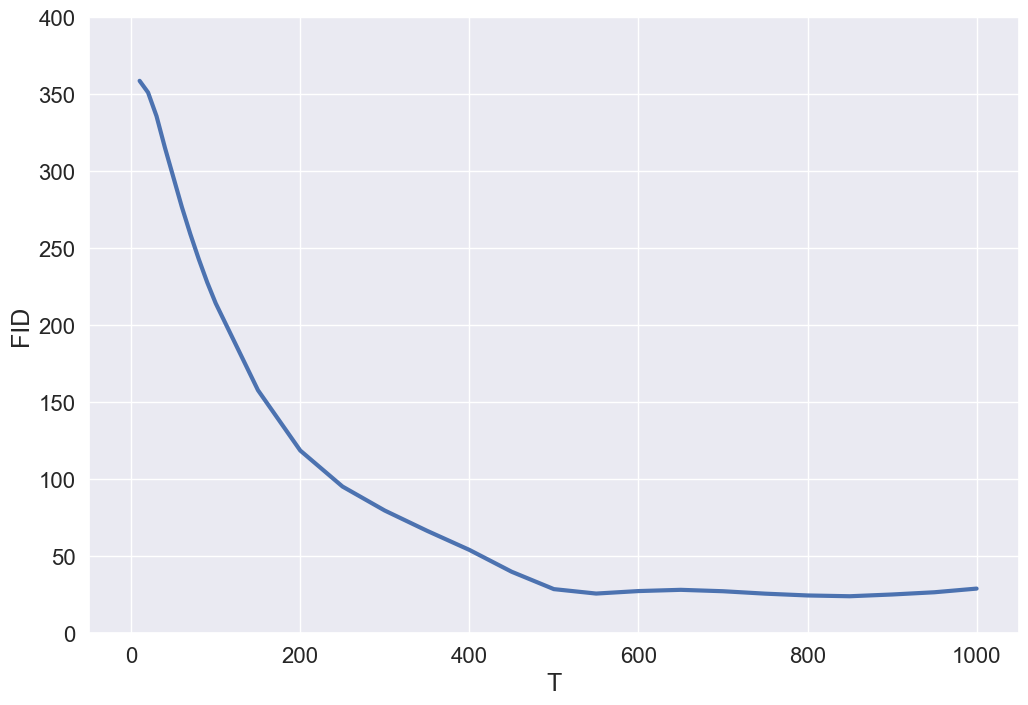
\includegraphics[scale=0.37]{figures/DDPM_FID_FMNIST.png}}
				 	\end{figure}
			 	\end{block}
			\end{column}
			\begin{column}{0.23\textwidth}
					\begin{figure}[H]
						\subfloat[T = 50]{%
							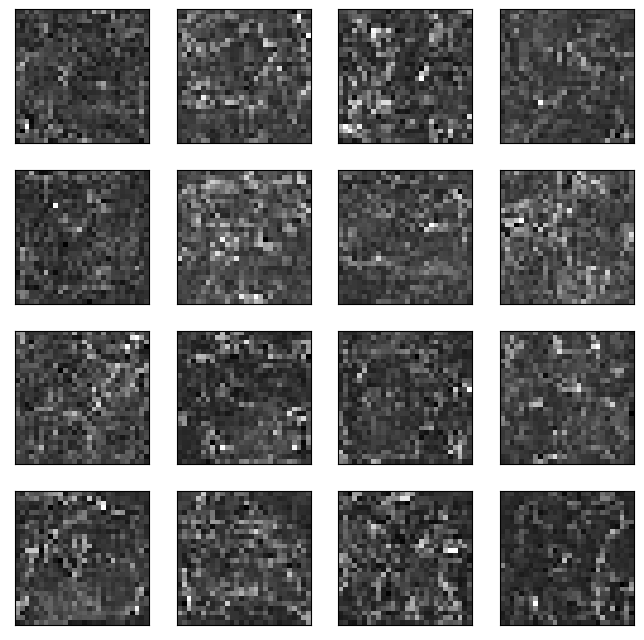
\includegraphics[width=0.8\columnwidth]{figures/generated_DDPM_50.png}}
						
						\subfloat[T = 300]{%
							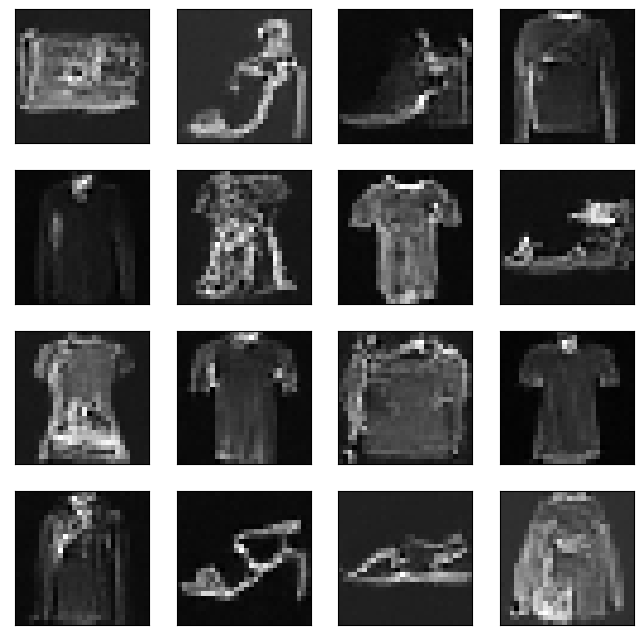
\includegraphics[width=0.8\columnwidth]{figures/generated_DDPM_300.png}}
					
						\subfloat[T = 1000]{%
							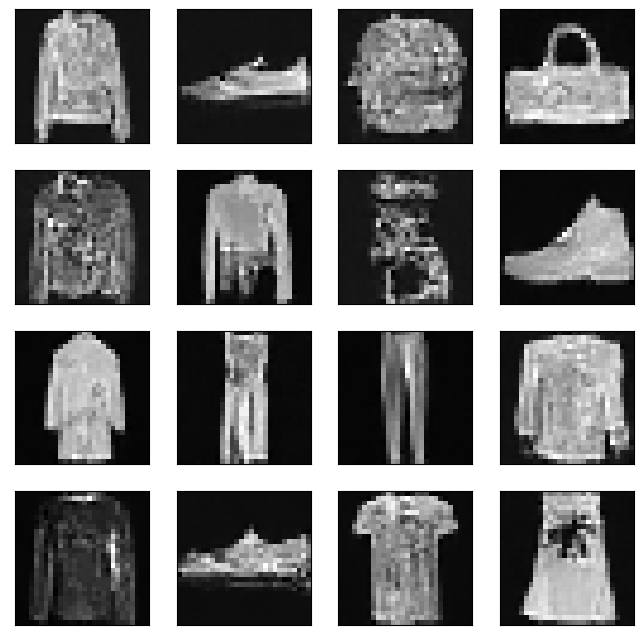
\includegraphics[width=0.8\columnwidth]{figures/generated_DDPM_1000.png}}
					\end{figure}	
			\end{column}
		\end{columns}
\end{frame}

\begin{frame}
	\frametitle{Вычислительный эксперимент}
	\begin{columns}
		\begin{column}{0.8\textwidth}
			\begin{block}{DDGAN с JS-дивергенцией}
				\begin{figure}[H]
					\centering{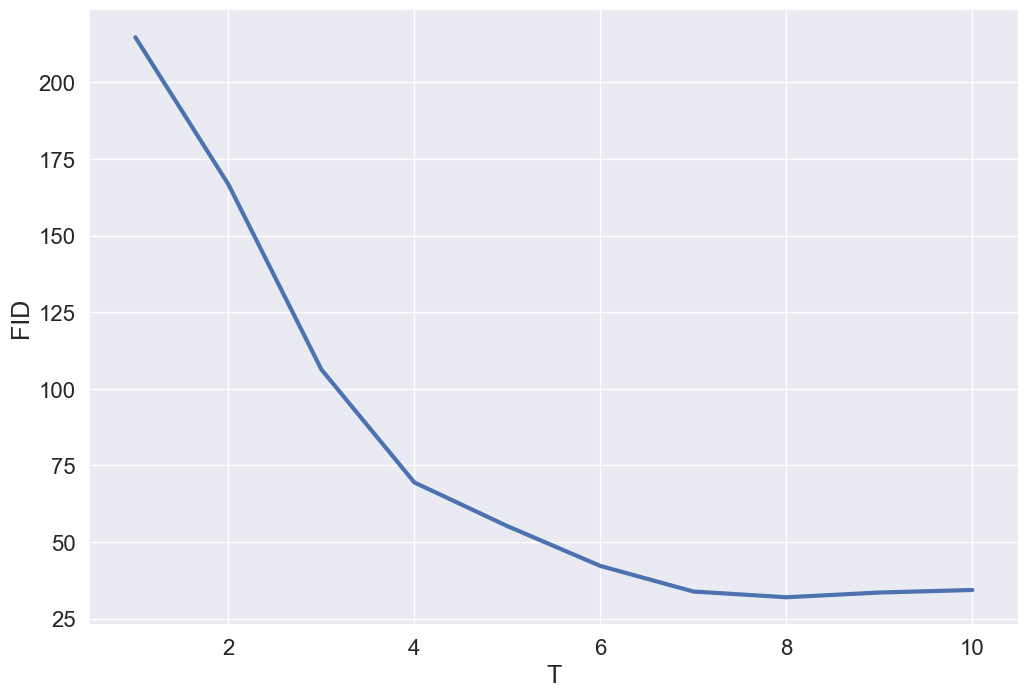
\includegraphics[scale=0.37]{figures/DDGAN_FID_FMNIST.png}}
				\end{figure}
			\end{block}
		\end{column}
		\begin{column}{0.23\textwidth}
			\begin{figure}[H]
				\subfloat[T = 3]{%
					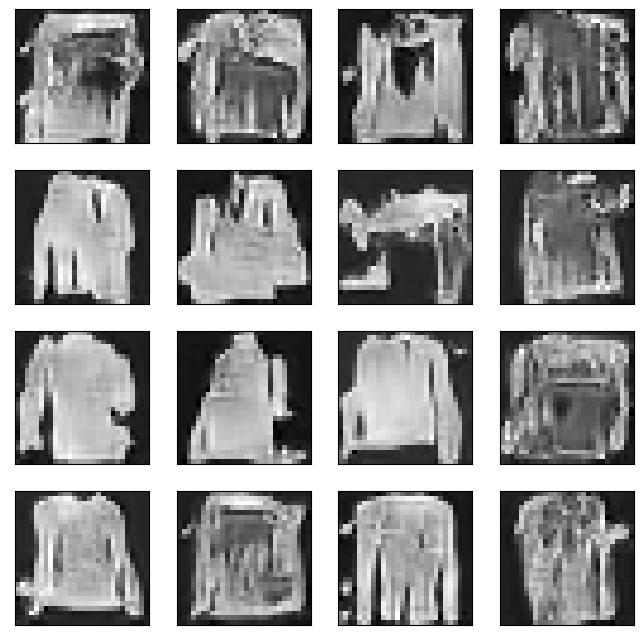
\includegraphics[width=0.8\columnwidth]{figures/generated_DDGAN_3.png}}
				
				\subfloat[T = 5]{%
					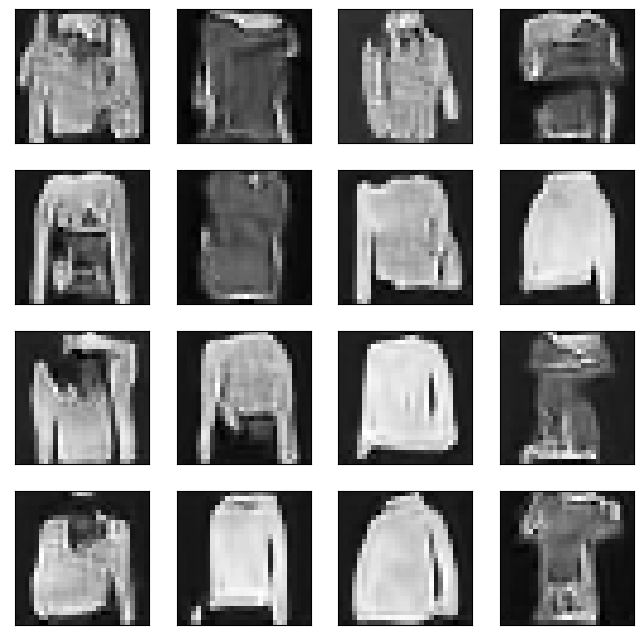
\includegraphics[width=0.8\columnwidth]{figures/generated_DDGAN_5.png}}
				
				\subfloat[T = 10]{%
					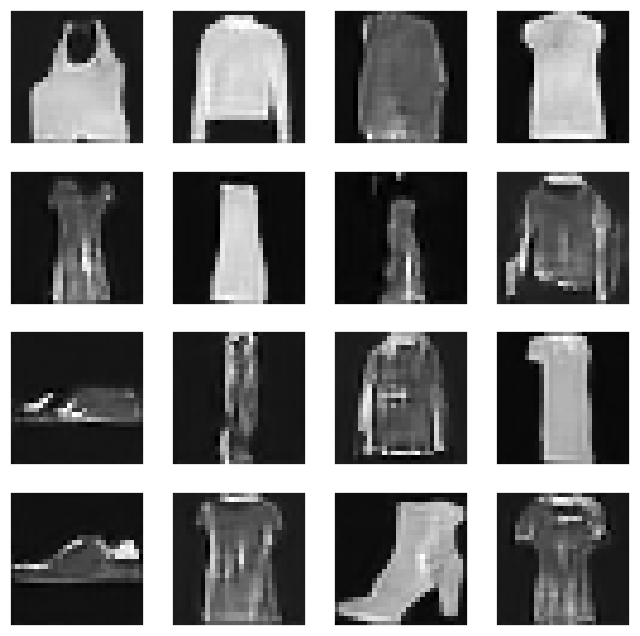
\includegraphics[width=0.8\columnwidth]{figures/generated_DDGAN_10.png}}
			\end{figure}	
		\end{column}
	\end{columns}
\end{frame}

\begin{frame}
	\frametitle{Вычислительный эксперимент}
	\begin{columns}
		\begin{column}{0.8\textwidth}
			\begin{block}{DDGAN с $H^2$}
				\begin{figure}[H]
					\centering{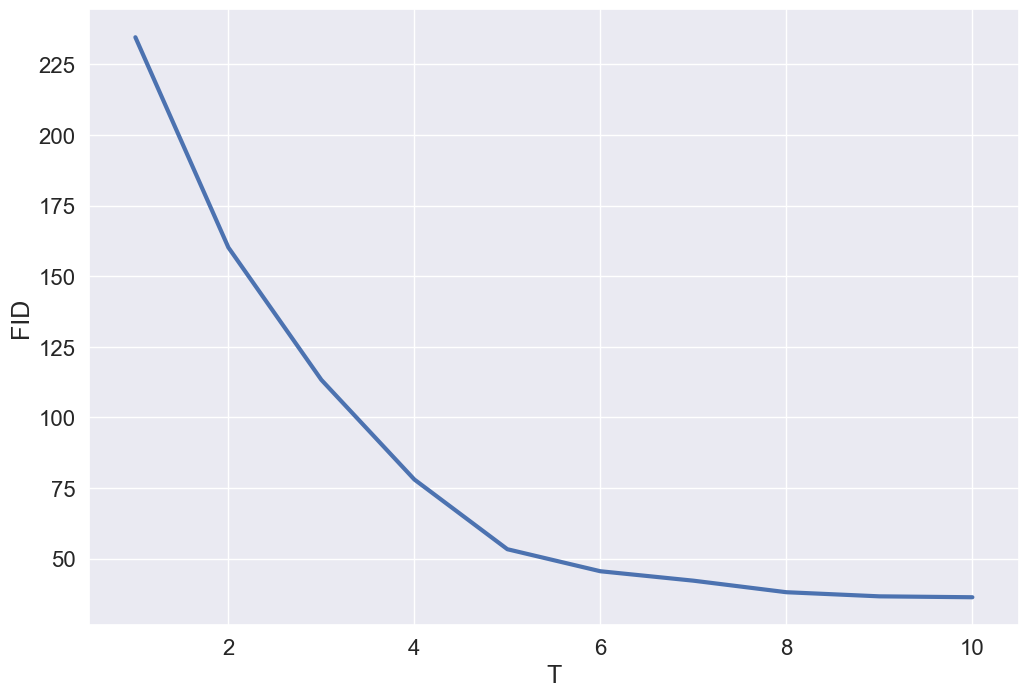
\includegraphics[scale=0.37]{figures/DDGAN_H2_FID_FMNIST.png}}
				\end{figure}
			\end{block}
		\end{column}
		\begin{column}{0.23\textwidth}
			\begin{figure}[H]
				\subfloat[T = 3]{%
					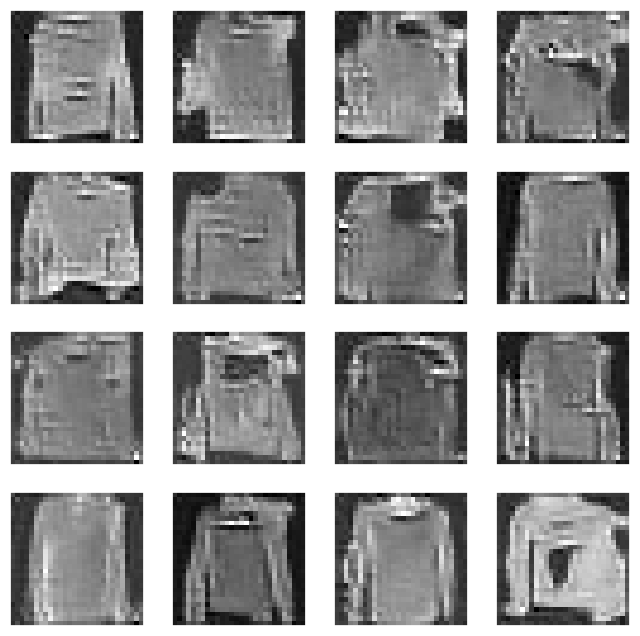
\includegraphics[width=0.8\columnwidth]{figures/generated_DDGAN_h2_3.png}}
				
				\subfloat[T = 5]{%
					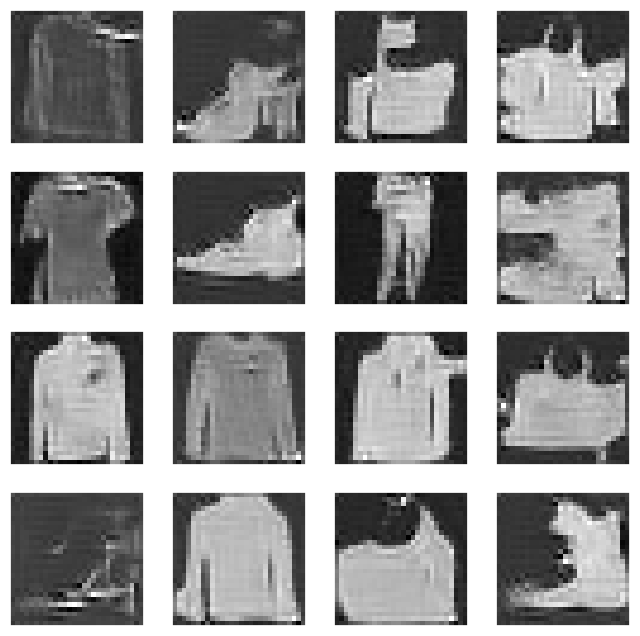
\includegraphics[width=0.8\columnwidth]{figures/generated_DDGAN_h2_5.png}}
				
				\subfloat[T = 10]{%
					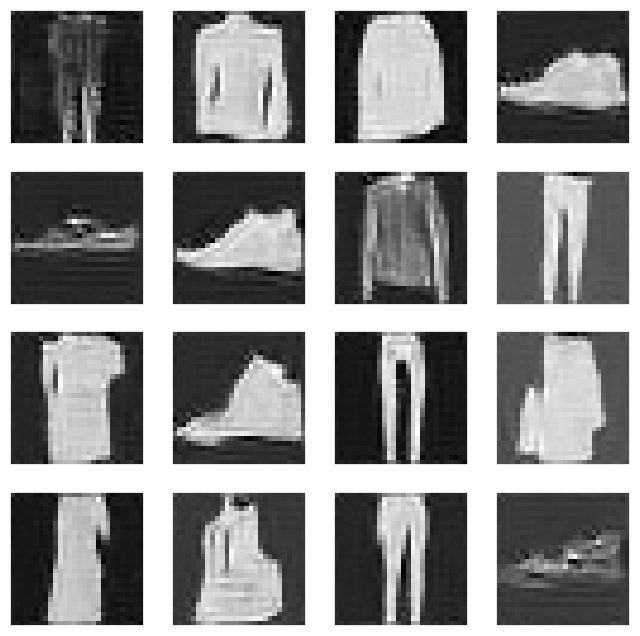
\includegraphics[width=0.8\columnwidth]{figures/generated_DDGAN_h2_10.png}}
			\end{figure}	
		\end{column}
	\end{columns}
\end{frame}

\begin{frame}
	\frametitle{Вычислительный эксперимент}
	\begin{columns}
		\begin{column}{0.8\textwidth}
			\begin{block}{DDGAN с обратной KL дивергенцией}
				\begin{figure}[H]
					\centering{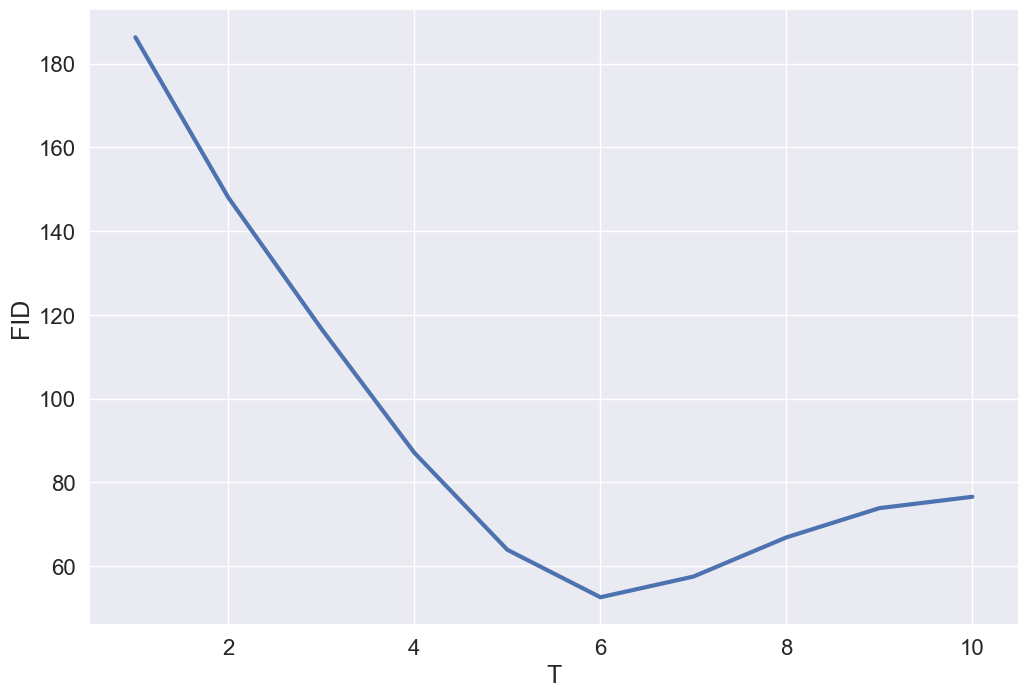
\includegraphics[scale=0.37]{figures/DDGAN_RKL_FID_FMNIST.png}}
				\end{figure}
			\end{block}
		\end{column}
		\begin{column}{0.23\textwidth}
			\begin{figure}[H]
				\subfloat[T = 3]{%
					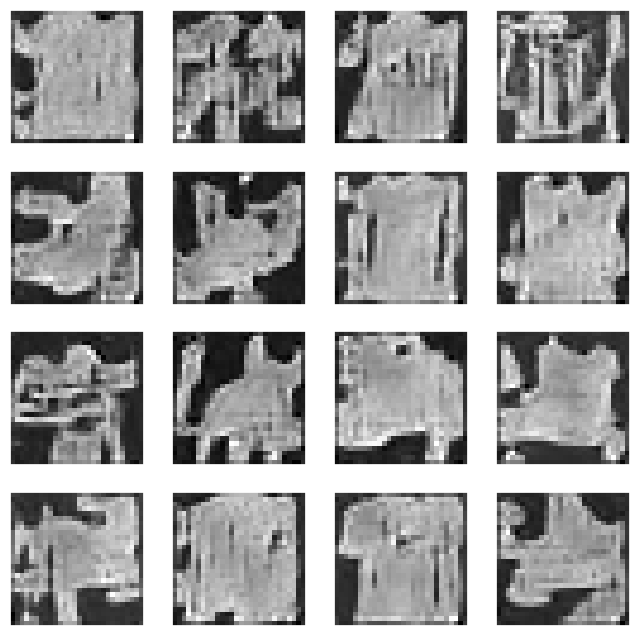
\includegraphics[width=0.8\columnwidth]{figures/generated_DDGAN_rkl_3.png}}
				
				\subfloat[T = 5]{%
					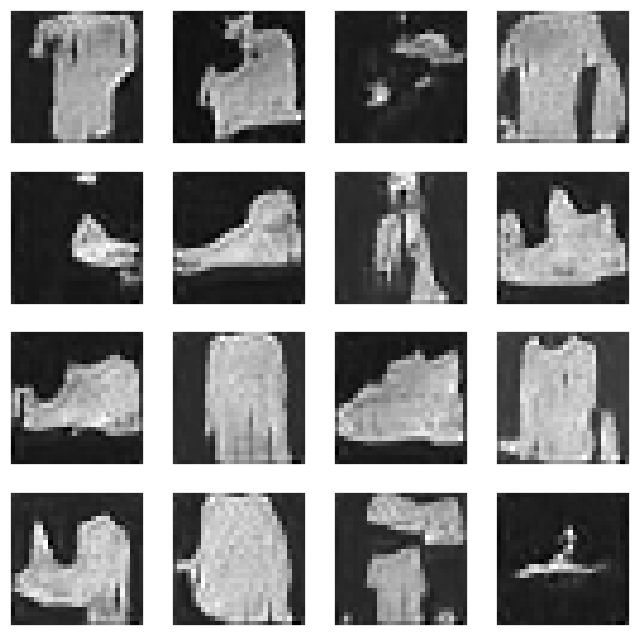
\includegraphics[width=0.8\columnwidth]{figures/generated_DDGAN_rkl_5.png}}
				
				\subfloat[T = 10]{%
					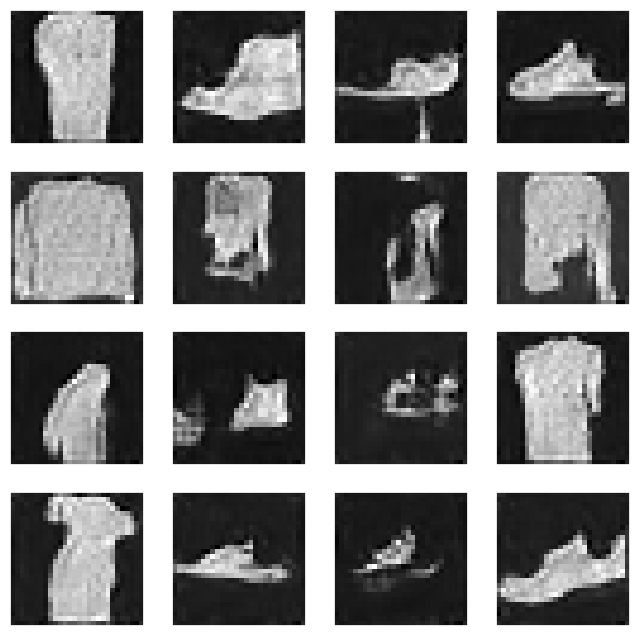
\includegraphics[width=0.8\columnwidth]{figures/generated_DDGAN_rkl_10.png}}
			\end{figure}	
		\end{column}
	\end{columns}
\end{frame}

\begin{frame}
	\frametitle{Вычислительный эксперимент}
	\begin{columns}
		\begin{column}{0.8\textwidth}
			\begin{block}{DDGAN с total variation}
				\begin{figure}[H]
					\centering{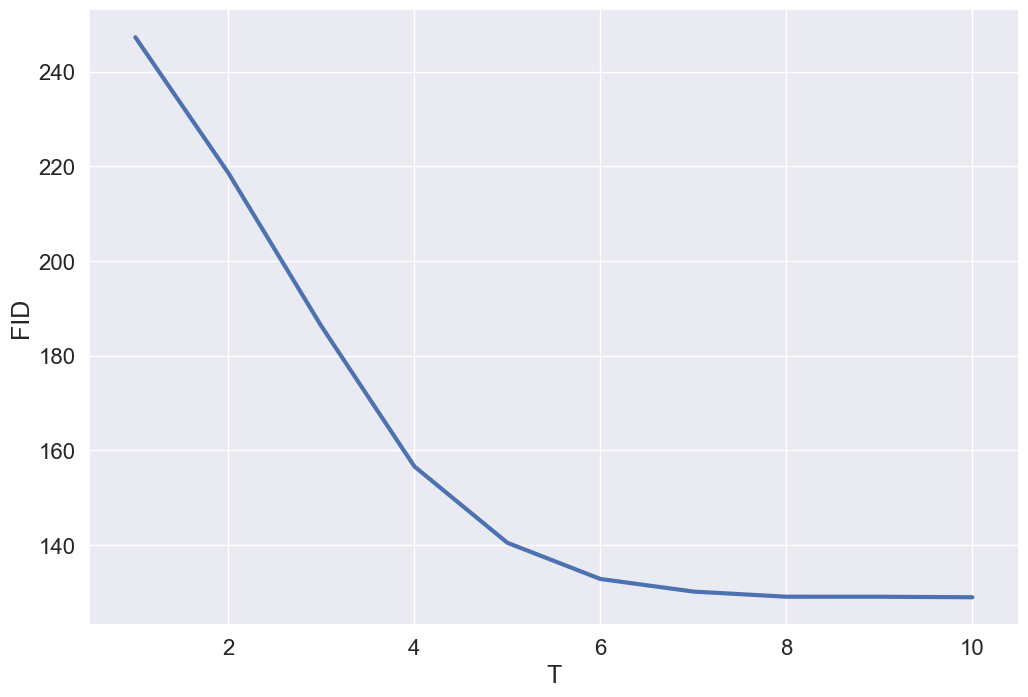
\includegraphics[scale=0.37]{figures/DDGAN_TV_FID_FMNIST.png}}
				\end{figure}
			\end{block}
		\end{column}
		\begin{column}{0.23\textwidth}
			\begin{figure}[H]
				\subfloat[T = 3]{%
					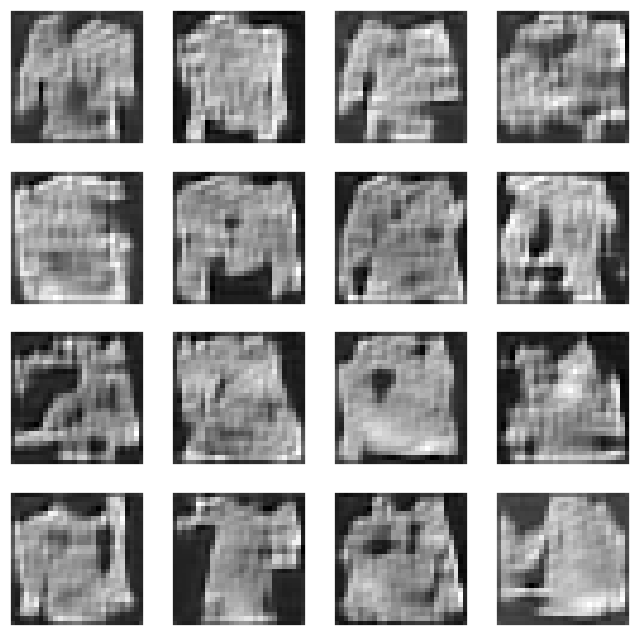
\includegraphics[width=0.8\columnwidth]{figures/generated_DDGAN_tv_3.png}}
				
				\subfloat[T = 5]{%
					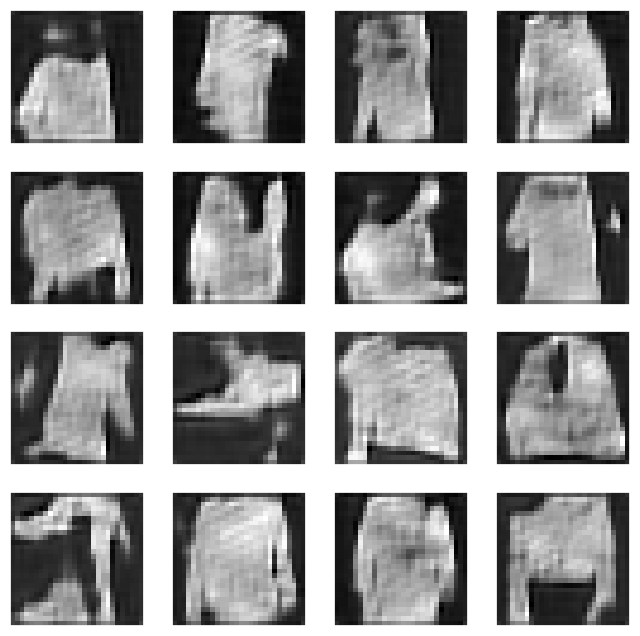
\includegraphics[width=0.8\columnwidth]{figures/generated_DDGAN_tv_5.png}}
				
				\subfloat[T = 10]{%
					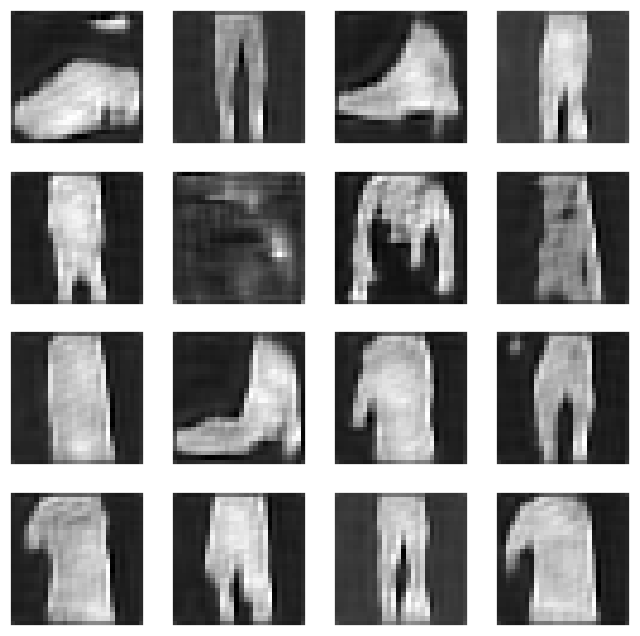
\includegraphics[width=0.8\columnwidth]{figures/generated_DDGAN_tv_10.png}}
			\end{figure}	
		\end{column}
	\end{columns}
\end{frame}

\begin{frame}
	\frametitle{Вычислительный эксперимент}
	\begin{columns}
		\begin{column}{0.8\textwidth}
			\begin{block}{DDGAN с wasserstein distance}
				\begin{figure}[H]
					\centering{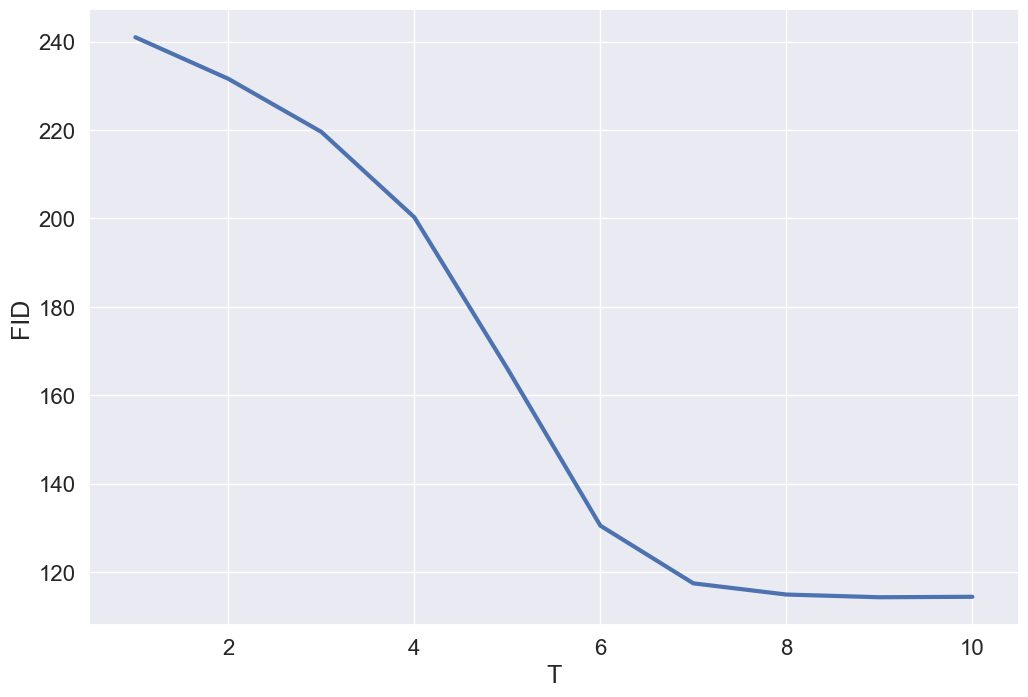
\includegraphics[scale=0.37]{figures/DDGAN_WD_FID_FMNIST.png}}
				\end{figure}
			\end{block}
		\end{column}
		\begin{column}{0.23\textwidth}
			\begin{figure}[H]
				\subfloat[T = 3]{%
					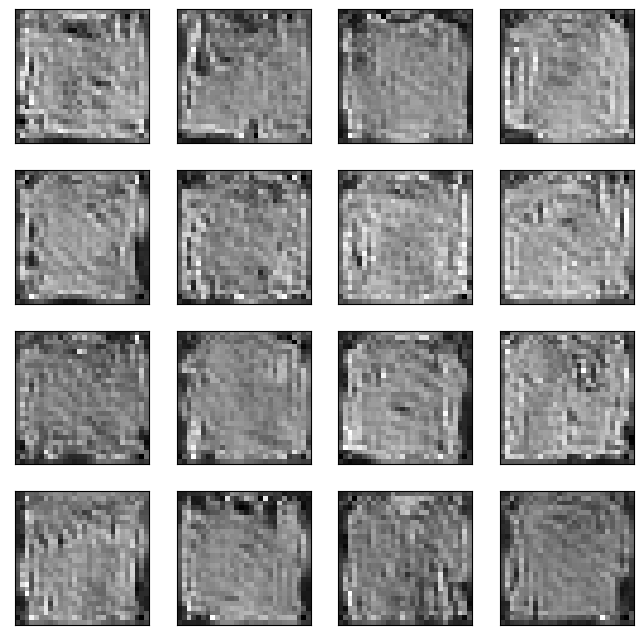
\includegraphics[width=0.8\columnwidth]{figures/generated_DDGAN_wd_3.png}}
				
				\subfloat[T = 5]{%
					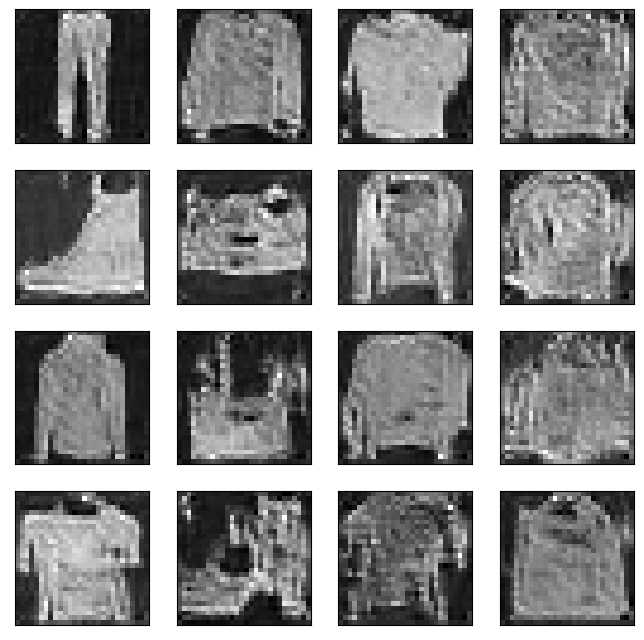
\includegraphics[width=0.8\columnwidth]{figures/generated_DDGAN_wd_5.png}}
				
				\subfloat[T = 10]{%
					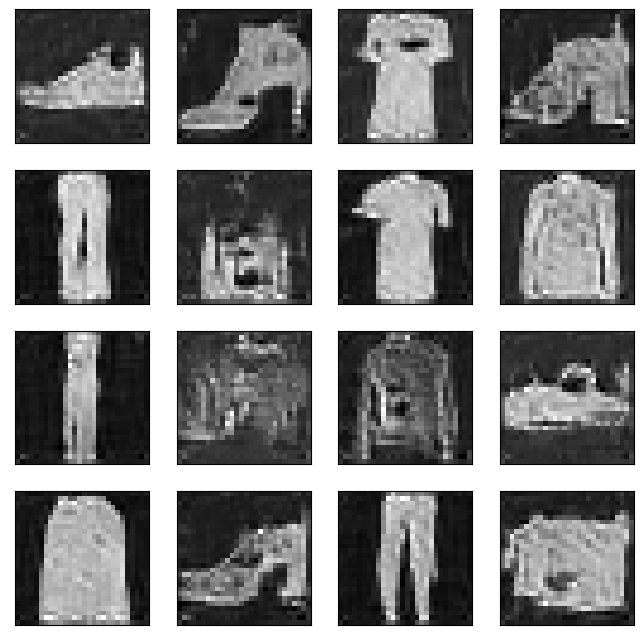
\includegraphics[width=0.8\columnwidth]{figures/generated_DDGAN_wd_10.png}}
			\end{figure}	
		\end{column}
	\end{columns}
\end{frame}

\begin{frame}
	\frametitle{Вычислительный эксперимент}
		\begin{block}{Сравнение различных схем тренировки}
			\begin{figure}[H]
					\centering{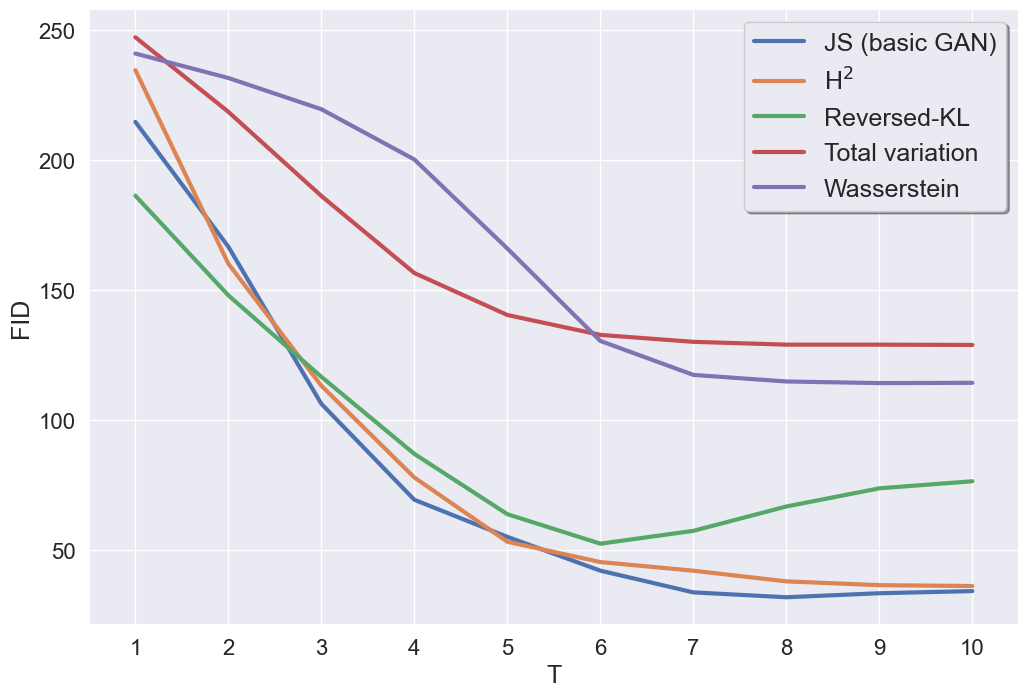
\includegraphics[scale=0.45]{figures/DDGAN_ALL_FID_FMNIST.png}}
			\end{figure}
		\end{block}
\end{frame}

\begin{frame}
	\frametitle{Вычислительный эксперимент}
	\begin{block}{Сравнение различных схем тренировки}
		\begin{longtable}{|c|c|}
			\hline
			Модель &  FID\\
			\hline
			DDPM &  28.9\\ 
			\hline
			JS DDGAN & 34.3 \\
			\hline
			H$^2$ DDGAN &  36.3\\
			\hline
			Reversed-KL DDGAN &  76.6\\
			\hline
			Total variation DDGAN &  129.0\\
			\hline
			Wasserstein DDGAN &  114.4\\
			\hline
			\caption*{FID-score для максимального T}
		\end{longtable}
	\end{block}
	\begin{block}{Итоги эксперимента}
		\begin{itemize}
			\item Количество шагов в диффузионной модели успешно снижено на 2 порядка при незначительном падении качества семплов
			\item Стандартный (JS) DDGAN показывает себя лучше остальных
			\item DDGAN с H$^2$ достигает сравнимого со стандартным качества
			\item Обучение всех DDGAN кроме стандартного склонно к разбалансировке и требует тщательного подбора гиперпараметров
		\end{itemize}
	\end{block}
\end{frame}

\begin{frame}
	\frametitle{Заключение}
	\FontUP
		\begin{itemize}
			\item Предложены различные способы моделирования мультимодального распределения в обратном диффузионном процессе
			\vfill
			\item Экспериментально подтверждена возможность использования различных подходов к обучению GAN моделей для использования их в диффузионной сети
			\vfill
			\item Проведено сравнение различных алгоритмов обучения на синтетических данных.
			\vfill
			\item В дальнейшем планируется исследовать способы выбора схемы тренировки в зависимости от входных данных
		\end{itemize}		
\end{frame}


\end{document}
